
To understand how many constraints are  specified in  software, where they are located, and what they are about, we wrote scripts to extract data constraints from the latest version of 
the 12 applications described in Section \ref{sec:meth}. Our scripts obtain a web application's Abstract Syntax Tree, check which Ruby validation APIs and migration APIs are used, and analyze their parameters.

In this paper, our script covers all types of constraints listed
in Table \ref{table:constraintdeftax} except for   
Custom sanity checks and raw SQL constraints. Both are rarely used in these
applications (e.g., raw SQL constraints are only specified in fewer than
30 times across all 12 applications). Note that, when we report inconsistency
or missing constraints, 
we manually check to make sure the inconsistency/missing constraint is not caused by
our script not covering these two types of constraints.

%Since it is impractical to automatically extract all custom sanity checks, we randomly sample some of the sanity checks and manually analyze them at the end of this section.

\subsection{How many constraints are there?}

\begin{table}
%\setlength{\tabcolsep}{1.2pt} 
\centering
\caption{\# Data constraints in web applications} 
\resizebox{0.7\columnwidth}{!}{
\begin{tabular}{lrrrrrrrrrrrr}

\toprule
 & Ds   & Lo  & Gi   & Re  & Sp  & Ro  & Fu & Tr  & Da  & On  & FF  & OS  \\
\midrule
DB   & 1403 & 137 & 1582 & 437 & 346 & 378 & 34 & 108 & 361 & 345 & 159 & 242 \\
App  & 165  & 33  & 496  & 220 & 132 & 219 & 13 & 30  & 116 & 82  & 17  & 176 \\
HTML & 0    & 2   & 18   & 32  & 0   & 0   & 0  & 2   & 1   & 11  & 0   & 0   \\
\midrule
Total  & 1568 & 172 & 2096 & 689 & 478 & 597 & 47 & 140 & 478 & 438 & 176 & 418\\
\midrule
\midrule 
LoC  & 62k & 11k & 122k & 35k & 31k & 17k & 1.7k & 13k & 21k & 14k & 7.8k & 14k
 \\
\midrule
\midrule 
\#Col   & 1180 & 150  & 1384 & 338  & 456  & 384  & 53   & 107  & 510  & 268  & 171  & 228  \\
\#Col$_\text{C}$ & 882  & 104  & 1140 & 297  & 312  & 272  & 32   & 82   & 348  & 228  & 146  & 174  \\
\%Col$_\text{C}$ & 75\% & 69\% & 82\% & 88\% & 68\% & 71\% & 60\% & 77\% & 68\% & 85\% & 85\% & 76\%\\
\bottomrule
\end{tabular}
}

{\footnotesize LoC: Lines of code. \#Col: number of data columns stored in the database. \\
\#Col$_\text{C}$.: number of columns associated with constraints.
Custom sanity check not considered.
}
\label{table:latestconstraintnum}
\end{table}

As shown in Table \ref{table:latestconstraintnum}, there are many constraints in these applications. 
%Naturally, the larger the software is and the more data columns the software contains, the more constraints are specified. 
Across all applications, 60\% - 88\% of data columns are associated with constraints and there exists 1.1 to 3.6 constraint specifications for every 100 lines of code.

\paragraph{\bf Summary} Data constraint specification widely exists in all types of web applications. Their consistency, maintenance, and handling affect the majority of the application data.


\subsection{Where are the constraints?}
\label{sec:one_where}

As shown in Table \ref{table:latestconstraintnum}, DB constraints are the most common, contributing to
58--90\% of all the constraints. Application constraints contribute 10--42\%, while front-end constraints are few.   
It is surprising that the number of DB constraints differs significantly compared to
application constraints, as both are supposed to be applied to a given piece of persistent data (Section \ref{sec:back_constraints}). Furthermore, inconsistencies
between them can lead to application crashes as in the example shown in Figure~\ref{fig:crossstack}. 
This led to the next few study items.

\paragraph{\bf What DB constraints are missing in applications?}
Table~\ref{table:dbpresentmodelmissingbreakdown} examines over
4,000 DB constraints that are missing in applications.

Alarmingly, about one quarter of these missing constraints (more than 1,000 in total)  involve string/text
data where developers did not specify any length constraints in the application, 
yet length constraints are imposed by the DB.
For example, 
whenever creating a table column of type ``string'' using Rails migration API, by default, Rails framework forces a length constraint of 255-character in the database, yet many of these string fields have no length constraints specified through application validation functions.
%Another example is MySQL has a default length constraint (no more than 65535 characters) on column of type ``text'', and applications often do not have the corresponding length limit. 
%when MySQL is the DB engine, all {\it text} fields 
%have 65535-character length constraint by default, and
%all {\it string} fields have 255-character length constraint
%by default set by the Rails migration API that adds or removes tables, columns, or entries \alvin{what's the migration api for?} \junwen{migration api is used to create db or alter db, they will be translated to sql queries to create/alter table}
%regardless of the databaseengine type.\junwen{Before Rails 4, 255 is for every engine, after Rails 4, 255 is only for MySQL} 
This mismatch could lead to severe problems: if a user tries to submit a long
paragraph/article in such a seemingly limitless field, his application will crash due to a failed {\tt INSERT} query, as shown in Figure~\ref{fig:crossstack}. In fact, we found many real-world issues reporting this problem (Sec.~\ref{subsec:where}), ultimately leading to developers adding the corresponding constraints in the application layer.

About 2\% of the missing constraints, 101 in total across the 12 applications, are associated with data fields that do not exist in the application.
Some of them are updated and read through 
external scripts, but never through the web application; 
others are deprecated fields that have already been removed
from the application but not dropped yet from the DB. 
Although this does not lead to immediate software misbehavior, 
these cases reflect challenges in
data maintenance and could cause functionality problems in the future. In addition,
they cause performance problems as the database needs to maintain deprecated data.

About one third of the missing constraints are automatically satisfied by Rails or the DB and are hence benign. This includes presence and numericality constraints associated with foreign-key fields (``ForeignKey''): 
foreign key fields are automatically generated
by Rails and satisfy presence
and numericality constraints in the DB. Meanwhile, there are also constraints that are guaranteed by the DB (``SelfSatisfied''), like presence constraints guaranteed by non-null default values specified in the DB, uniqueness constraints guaranteed by an auto-increment property in the DB, etc.

\begin{table}
\centering
\caption{\# Constraints in DB but not in Application} 
\setlength{\tabcolsep}{2pt}  
\resizebox{0.7\columnwidth}{!}{
\begin{tabular}{lrrrrrrrrrrrrr}

\toprule
& Ds   & Lo  & Gi   & Re  & Sp  & Ro  & Fu & Tr  & Da  & On  & FF  & OS & All \\
\midrule
StrLength & 243 & 21 & 406 & 49 & 182 & 47 & 18 & 21 & 101 & 69 & 74 & 28 & 1259 (28\%) \\ \midrule
AbsentData & 21 & 0 & 40 & 2 & 2 & 2 & 2 & 1 & 22 & 7 & 2 & 0 & 101 (2\%) \\ 
\midrule
ForeignKey & 266 & 31 & 271 & 82 & 27 & 99 & 7 & 27 & 61 & 91 & 16 & 30 & 1008 (22\%) \\ \midrule
SelfSatisfied & 192 & 16 & 161 & 84 & 28 & 9 & 2 & 18 & 3 & 20 & 8 & 31 & 572 (13\%) \\ \midrule
Others   & 446 & 39 & 429 & 126 & 77 & 89 & 2 & 29 & 143 & 82 & 26 & 64 & 1552 (35\%) \\
\bottomrule
\end{tabular}
}
\label{table:dbpresentmodelmissingbreakdown}
\end{table}

\begin{table}
\centering
\setlength{\tabcolsep}{1.5pt}  
\caption{\# Constraints in Application but not in DB }
{\textmd{(only
built-in validation constraints are listed)}}
 
\resizebox{0.7\columnwidth}{!}{
\begin{tabular}{lrrrrrrrrrrrrr}

\toprule
& Ds   & Lo  & Gi   & Re  & Sp  & Ro  & Fu & Tr  & Da  & On  & FF  & OS & All \\
\midrule
Presence & 8 & 5 & 37 & 15 & 38 & 49 & 5 & 5 & 34 & 3 & 1 & 9 & 209 (51\%) \\ \midrule
Unique & 3 & 1 & 12 & 18 & 19 & 5 & 0 & 4 & 16 & 1 & 0 & 9 & 88 (21\%) \\ 
\midrule
Inclusion/Exclusion & 7 & 1 & 13 & 11 & 2 & 0 & 2 & 0 & 7 & 5 & 0 & 9 & 57 (14\%) \\ \midrule
RegEx & 8 & 5 & 10 & 7 & 0 & 9 & 0 & 0 & 11 & 4 & 0 & 3 & 57 (14\%) \\ \midrule
%Other   & 15 & 2 & 3 & 9 & 13 & 1 & 0 & 0 & 3 & 0 & 2 & 10 & 58 (11\%) \\
Numeric   & 0 & 0 & 0 & 0 & 0 & 1 & 0 & 0 & 0 & 0 & 0 & 0 & 1 (0.2\%) \\ 
\bottomrule
\end{tabular}
}
\label{table:modelpresentdbmissingbreakdown}
\end{table}

The remaining one third of the constraints ("other") are difficult to analyze automatically. Based on our manual sampling and checking, most  
are already satisfied by how the application processes and generates corresponding data fields. 
Although they do not cause problems currently, developers should nonetheless be informed about them, so that code changes can be tested
against these constraints to prevent regression failures. 

\underline{\it False-positive analysis}\ \ Besides the ``Others'' row in Table \ref{table:dbpresentmodelmissingbreakdown},  
the other 4 rows are counted by our static-checking script. 
To check the accuracy of our script,
we randomly examined 102 cases from these 4 rows.
Among these cases, we found 7 false positives: 5 are not
DB constraints but are mistakenly identified due to syntax not handled by our script; 2 ``StrLength'' cases  
actually belong to ``Others,'' as the length requirement is guaranteed
by application semantics. These 102 cases include 58 ``StrLength''
cases, among which 5 are false positives --- 3 are not
DB constraints and 2 belong to ``Others''. %\junwen{Utsav, can you update the value here.}

\paragraph{\bf Which application constraints are not in database?}
Nearly 25\% of the constraints specified through application validation are missing in the DB.  
Table \ref{table:modelpresentdbmissingbreakdown}
breaks down the ones specified through built-in validation 
functions based on the constraint type
(412 in total). 
These missing constraints allow users to directly
change persistent data using SQL queries in ways that are disallowed by the application, causing functionality or even security problems.\footnote{It is common that database administrators directly change database data using queries and scripts, bypassing the application server.} Furthermore, some of these missing constraints represent missed query optimization opportunities, such as improving cardinality estimation in query plan generation using such constraints~\cite{lohmanBlog}.

About half of these missing constraints
are presence constraints. That is, a field $f$ is required to be non-null in the application, but is not required so in the DB --- their default values are ironically set to be null in the DB. 
When users or administrators directly insert records into the DB without specifying the value
for a field $f$, the DB would accept these records and put null into $f$. 
Subsequently, when such records are retrieved and used in the application that 
assumes all $f$ to be non-null, software failures could occur.

Another category of missing constraints that can easily cause problems are uniqueness constraints. Without being
specified in the DB, a uniqueness constraint often {\bf cannot} be guaranteed by the application \cite{perilsofuniqueness,uniquenessrb}: 
web users could make concurrent update requests that save duplicate values into the DB, violating the uniqueness constraint and causing software failures and maintenance challenges. 
%(the discovery and cleanup of bad data).
%\utsav{Rails uses transactions on save by default, but I think the isolation level, at least for Postgres, is READ COMMITTED which may not prevent against this. Anyway it may happen infrequently in practice, but there are warnings about this in the rails documentation https://github.com/rails/rails/blob/master/activerecord/lib/active\_record/validations/uniqueness.rb\#L165, and in blog posts: https://thoughtbot.com/blog/the-perils-of-uniqueness-validations}


Regular expression and inclusion/exclusion constraints are rarely found in the DB layer. While these can be enforced via procedures or {\tt ENUM} types, they are not natively supported by the Rails DB migration APIs and have to be explicitly specified via SQL, which might be a reason why they tend to be missed in the DB.
Inclusion/exclusion 
constraints limit the value of a field to a small set of
constants and would be very useful in avoiding data corruption, saving storage space, and improving database performance (e.g.,
through DB selectivity optimization) if they are present.

The single numeric constraint in Table \ref{table:modelpresentdbmissingbreakdown} is a ``phone number'' field that is
specified to be numeric in application but stored as a ``string'' in the database.

\underline{\it False-positive analysis}
 We randomly sampled
and examined 10 cases from each of the 4 main categories in Table \ref{table:modelpresentdbmissingbreakdown} (Presence, Unique,
In/Ex-clusion, RegEx).  
3 out of the 40 sampled cases are false positives 
(2, 0, 0, 1 in the 4 categories, respectively)---syntax corner cases caused our script to identify 1 spurious presence constraint, and the remaining 2 are related to conditional constraints.

\paragraph{\bf Summary} Hundreds and thousands of database constraints do not exist
in application, and vice versa. The majority of these discrepancies can actually
lead to bad user experience (missing string length constraints),   
database maintenance challenges (data fields that are no longer used in the application),
code maintenance challenges (constraints implicitly guaranteed by the application logic),
data corruptions, software failures, or sub-optimal database performance (missing DB constraints). They can be avoided by implementing constraints in the application and as SQL constraints in the database. However, in practice inconsistencies are likely inevitable if we only rely on developers' manual effort.
It would be helpful to develop automated techniques that coordinate
database and application constraints.

\subsection{What types of constraints are there?} 
\paragraph{\bf Standard types}
Table~\ref{table:apibreakdown} shows the most popular constraint types among all front-end, application built-in validation, and DB constraints. 
The top 2 most popular types are consistently presence and length.
%The much smaller number of Numericality constraints in Application is due to the fact that numericality constraints for foreign-key fields are implicitly enforced by Rails and hence not specified in application.
%None of the 86 Inclusion application constraints exist in the DB, as discussed earlier.


\begin{table}[]
\caption{Top 5 popular types of different layer}

\resizebox{0.7\columnwidth}{!}{
\begin{tabular}{@{}llllll@{}}
\toprule
DB  &   Presence & Length &  Numericality&  Uniqueness   & -         \\ \midrule
 &  1822 (32.9\%)        & 1784 (32.3\%)      & 1650 (29.8\%)              & 276 (5.0\%)              & -         \\ \midrule
App. & Presence & Length & Uniqueness   & Numericality & Inclusion \\ \midrule
 & 888 (52.3\%)         & 218 (12.8\%)       & 209 (12.3\%)             & 101 (5.9\%)              & 67 (3.9\%)       \\ \midrule
HTML  & Presence & Length & Format       & -            & -         \\ \midrule
    &52 (78.8\%)          & 11 (16.7\%)        & 3 (4.5\%)         &            -  &      -     \\ %\midrule
%Sum   & Presence & Length & Numericality & Uniqueness   & Inclusion \\ \midrule
%      & 2822     & 1780   & 1492         & 414          & 77        \\ 
\bottomrule
\end{tabular}
}
\label{table:apibreakdown}
\end{table}


\paragraph{\bf Custom validation constraint types}
Custom validation functions are used much less often than built-in ones,
but are not rare, contributing about 5\% to slightly over 25\% of all application
validation functions across the 12 applications (avg. 18\% across all apps). 
%To understand what types of custom constraints are specified, 
We randomly sampled 50 custom validation functions
and found that more than half of them are used to check multiple fields at the same time (27 out of 50), like the function {\tt presence\_of\_content} in the
{\tt StatusMessage} model from {\tt Diaspora}, which requires that at least one of the fields {\tt text} or {\tt photos} be non-empty. 
%In some cases (11 out of 50), the condition checking involves data in DB tables used by the application but not directly associated with the model, or data from the application configuration. \shan{this table is not managed by the web application?}\utsav{Tried to clarify} 
These custom validations seldom have corresponding constraints in DB --- only 4 out of the 50 we sampled exist in DB.  

\iffalse 
\begin{table}[h]
\caption{\# Custom validation constraints (sample size: 50)}
\setlength{\tabcolsep}{2pt}  
\footnotesize
%@{\hspace{0.3in}}r@{\hspace{0.3in}}r@{\hspace{0.3in}}r@{\hspace{0.3in}}r@{\hspace{0.3in}
\resizebox{0.9\columnwidth}{!}{
\begin{tabular}{rrrr}
\toprule
 Multi-field & Pre-processing & External data & Other \\
\midrule
27 & 6 & 11 & 16 \\
\bottomrule
\end{tabular}
}
\label{table:custommethodmulti}
\label{table:issueapp}

{\footnotesize Note that some custom validators contain multiple functionalities.}
\end{table}
\fi 




\iffalse
\begin{figure}[h] 
    \centering
    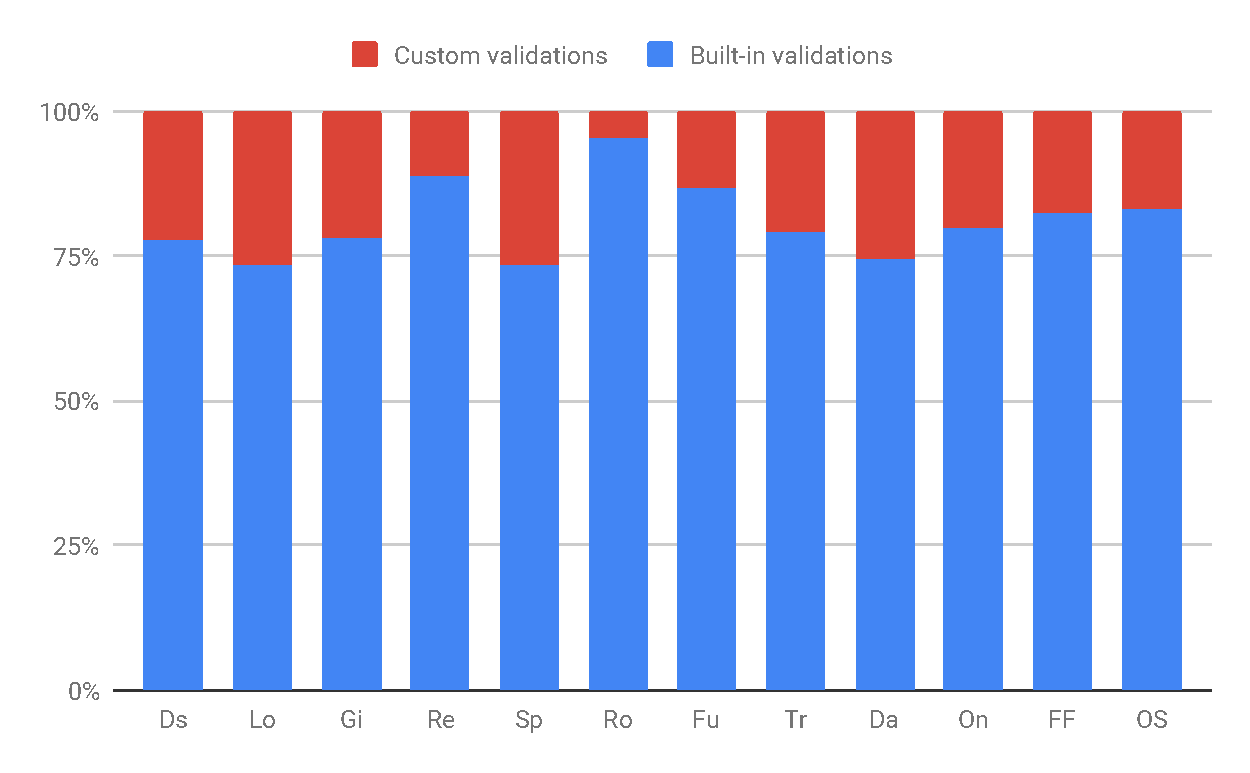
\includegraphics[width=\columnwidth]{figs/custom-vs-builtin-validations.pdf}
    \caption{Breakdown of \# of custom vs. built-in validations in model layer
\\  \junwen{change to a table?}
}
    \label{fig:model-breakdown}
\end{figure}
\fi 


\paragraph{\bf Custom sanity check types}

We also sampled 20 sanity checks on input parameters from the controller code of 5 applications.
%\shan{are these in one application or multiple? }
Among these 20 checks, the majority (17) are indeed checking inputs  that are related to persistent
data stored in the DB. Among these 17, 5 are about
data constraints, including presence and inclusion constraints, 
while the others are related to conditional data update/re-processing.
 Among these 5 constraints, only 1 is specified
in an application validation function and none exists in the DB.
%this 1 case is an inclusion constraint  

\iffalse 
\begin{table}[h]
\caption{\# Param sanity checking w/ category (sample size: 20)}
\footnotesize
\begin{tabular}{@{\hspace{0.1in}}r@{\hspace{0.2in}}r@{\hspace{0.2in}}r@{\hspace{0.2in}}r@{\hspace{0.1in}}}
\toprule
 Stored in DB & Constraint & Constrained in model & Constrained in DB\\
\midrule
17 & 5 & 1 & 0\\
\bottomrule
\end{tabular}
\label{table:nonapiconstraint}
\label{table:issueapp}

\end{table}
\fi 

\paragraph{\bf Summary} Although simple constraints like presence, length,
and numericality are the most common, more complicated constraints, such as those
involving multiple fields, are also widely used. Most of the
custom constraints are missing from the DB, while constraints reflected by sanity checks are often missing in both the application and DB. 
Future research that can automatically
reason about custom sanity checks and custom validation 
functions
%, which will likely require symbolic code evaluation,
can greatly help to identify and add missing constraints.